\chapter{System Model}

\section{Overview}
The iterative enhancement approach is a software development methodology that involves building a system incrementally while incorporating lessons learned from previous iterations. The process entails starting with a basic implementation of software requirements and gradually improving the system through successive iterations. Each iteration involves adding new functional capabilities to the design. For the development of a website, it is essential to define the project requirements, create a backlog of tasks, and prioritize them based on importance and complexity. By adopting an Agile model, the developer can continually deliver new website features, ensure user satisfaction, and remain responsive to evolving requirements throughout the development process.\\
\begin{figure}[H]
    \centering
    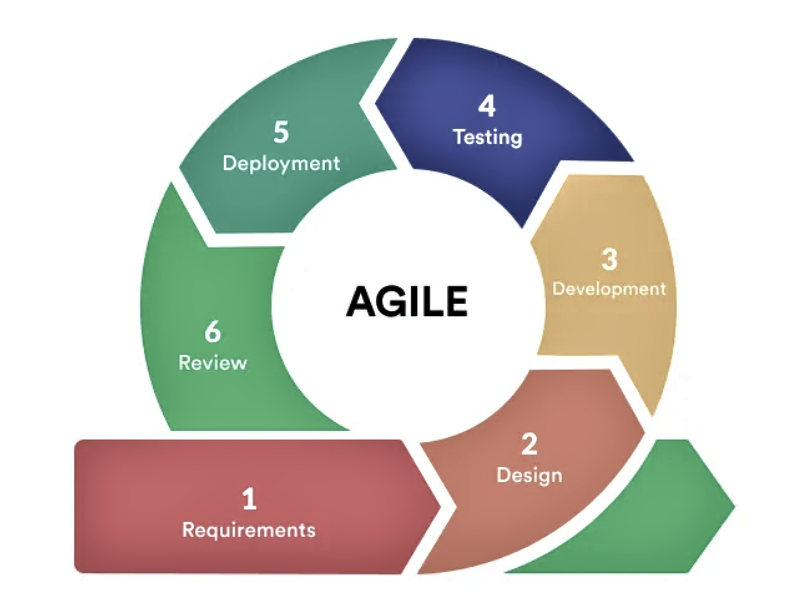
\includegraphics[scale=.6]{img/agile.png}
    \caption{The agile model}
    \label{fig:agile}
\end{figure}
The above model will help to build the web application step-by-step. This online system will help a university authority to follow up the department performance and it will be easier for both the users and admin panel. The students and the teachers will need to sign-up and login before enrolling in the system. The admin will check all the information provided by teachers and the students and also the admin will be responsible to give access to the account of them. For designing the process there have been used HTML, JavaScript and CSS and for the back-end and the database management Django and SQLite accordingly.\\


\section{Methodology}
Software performance guarantees that the application will function properly under a specific workload. The purpose of testing a system's performance is to confirm the responsiveness and functionality of particular features that were especially created for the system. Understanding how a software application behaves under a particular expected load and figuring out how resistant the application is under excessive stress are both crucial. Software performance demonstrates that the system satisfies the performance requirements. The system's burden or specific non-performing components can be found through performance testing. It is crucial for a new system's cost performance that attempts to create performance tests start as soon as the project is developed and continue as it moves forward. To understand better from both the teacher and student perspective here a picture is attached for understanding the whole process of this project.
\begin{figure}[H]
    \centering
    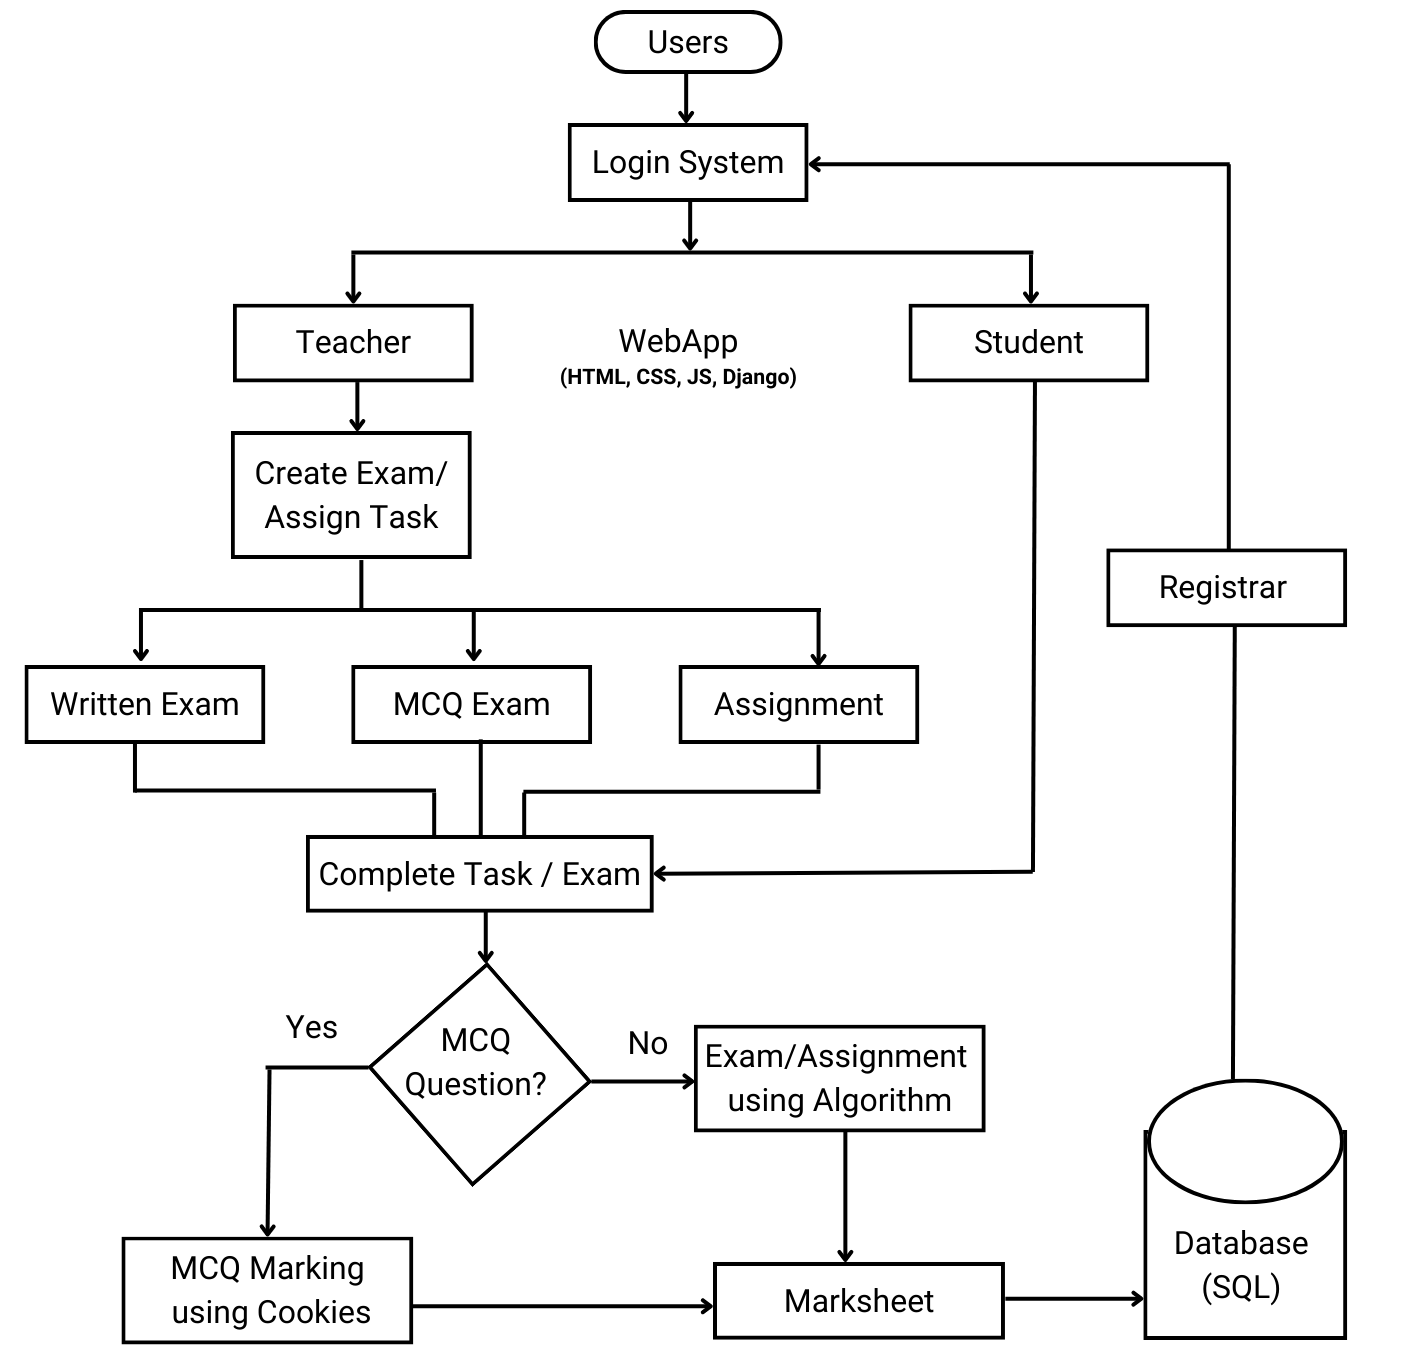
\includegraphics[scale=.36]{img/system-diagram.png}
    \caption{System Model}
    \label{fig:System}
\end{figure}
From the above figure \ref{fig:System} we can clearly understand that there will be two users to login into the system. The teacher will assign any kind of task which can be a mcq and written exam, assignment to the student and within a given period of time students will have to submit the task. MCQ exam will be evaluated or marked by the cookies of their local browsers and written exam or assignment will be evaluated by following machine learning algorithms. Then the assigned teacher will submit the marksheets of the students after evaluating. Finally the marksheet will be checked by the admin panel that means the registrar will check the final mark sheets from the database. \\

\section{System Design}
The system would require user authentication to ensure that only registered users, i.e. teachers and students, can access the system. A login page would be provided to the users, where they can enter their credentials to access the system. The system would have two types of users, teachers and students, each with their own set of permissions. Teachers would be able to create and assign tasks, evaluate submissions, and submit marksheets. Students would be able to view and attempt the assigned tasks, and submit their solutions. After evaluating the submissions, the teacher would be able to submit the marksheets of the students. The mark sheets would be stored in a database for further review. The admin panel, i.e. the registrar, would be able to access the database to review the final marksheets. The system would require a database to store the user information, tasks, submissions, and marksheets. The database would be managed using a database management system SQL. The system would be designed with security and privacy in mind. User data would be encrypted, and the system would use HTTPS for secure communication. User access would be restricted based on their roles and permissions, and regular backups would be taken to prevent data loss.

\subsection{Evaluation Process}
The online management system makes it possible to search and adds features like generating a task, approving the task, and letting the supervisor decide whether to accept the student or not. Both teachers and students' user profiles are kept up to date by the system administrator. The technology requires students to register an account before checking their credentials against faculty records. While it is necessary to take the class with the teacher, communication takes place by email. As it is said before, the evaluation process will be two types for evaluating the written types and mcq types.

\newpage
\subsubsection{Written Paper Mark Calculation}
The written ones will be checked for similarity by machine learning algorithms and marked accordingly. The process has been given below:\\

\begin{figure}[H]
    \centering
    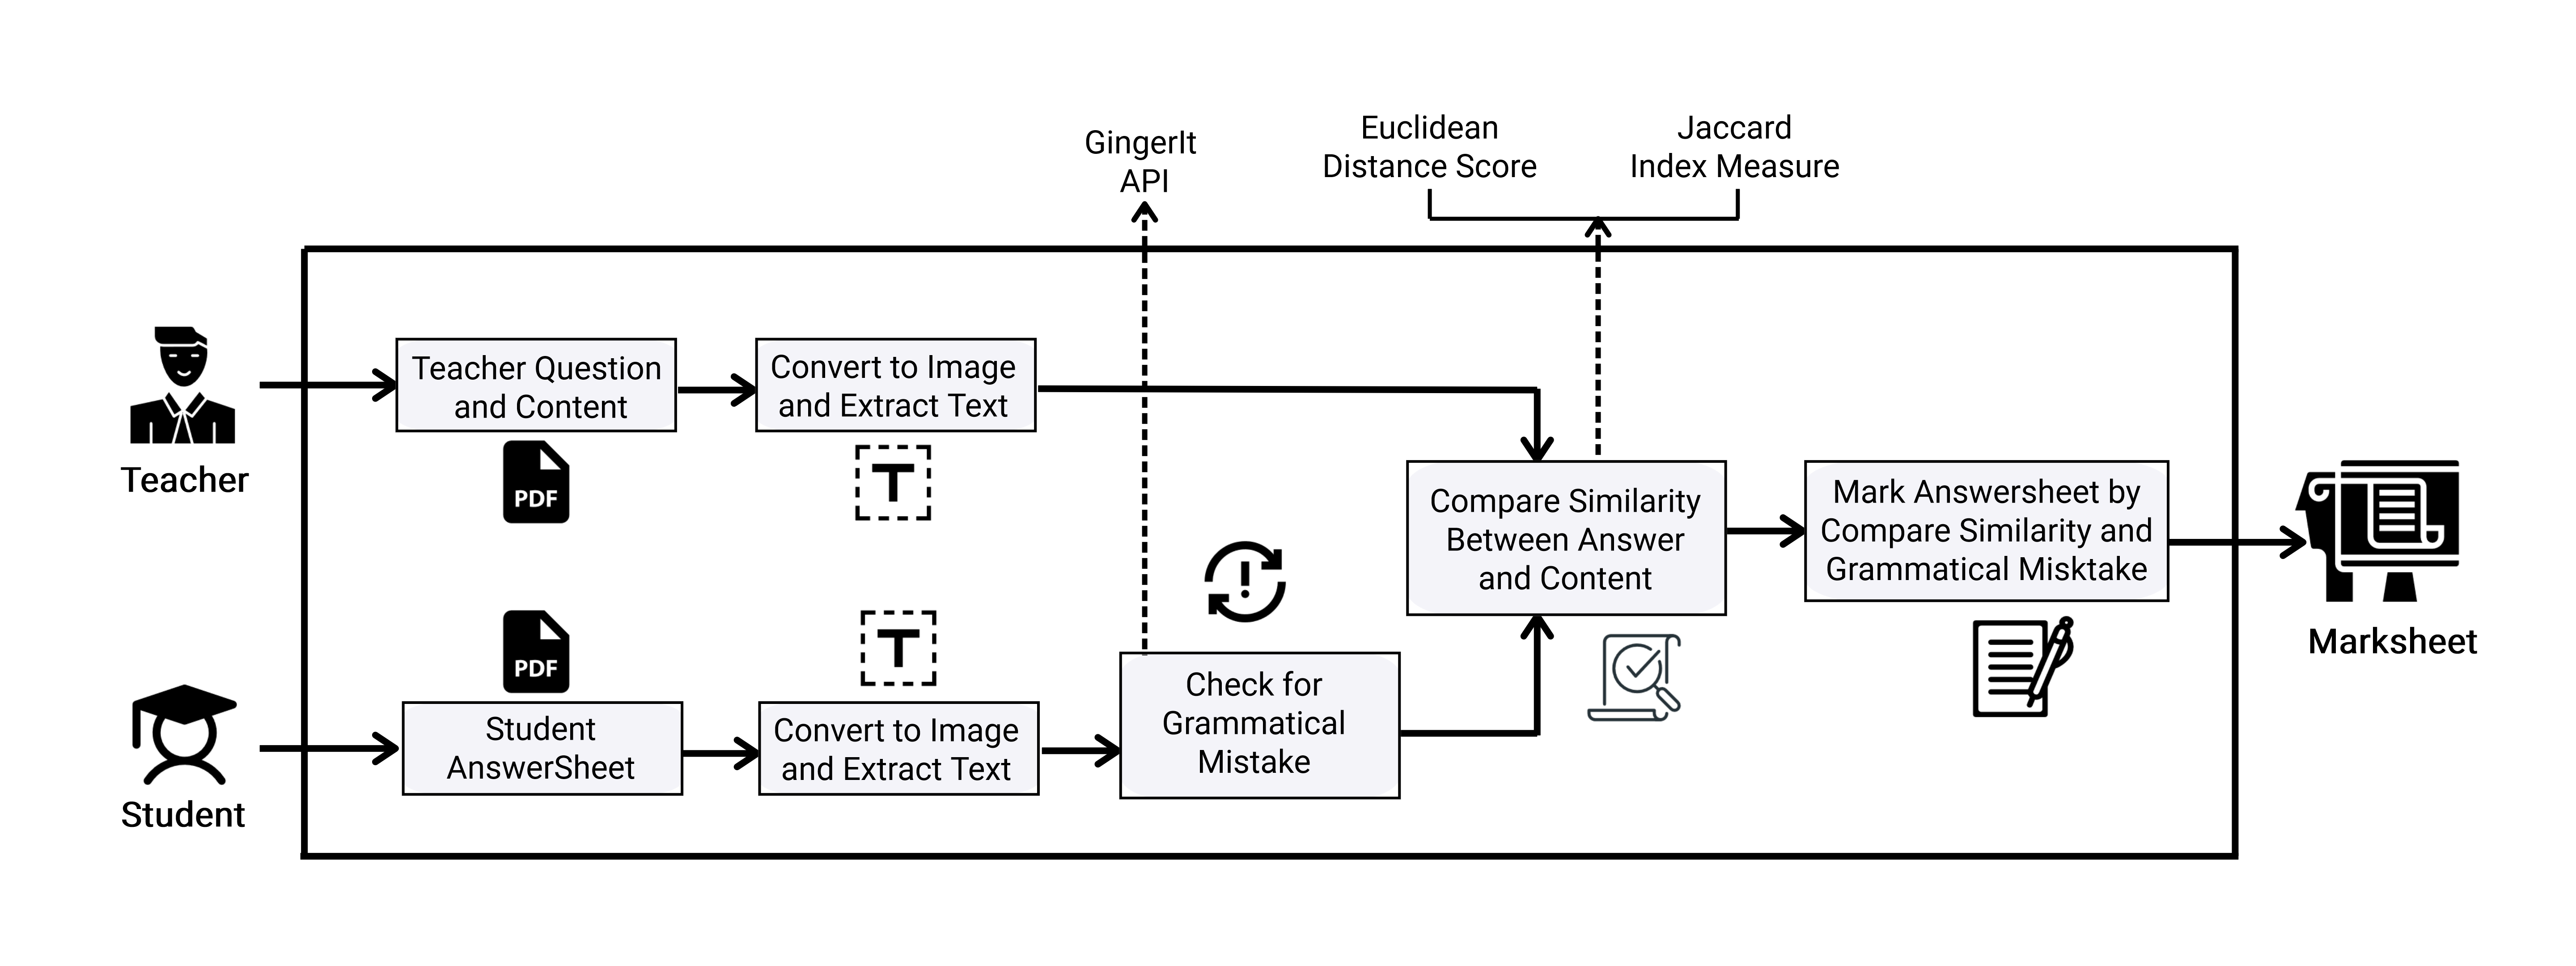
\includegraphics[scale=.07]{img/written.png}
    \caption{The written part evaluation process}
    \label{fig:written}
\end{figure}

In the above figure \ref{fig:written}it can be seen that after getting the answer sheet, the file will be converted into an image and we will need to extract the text. After that, the grammatical mistake will be checked and also the similarity will be checked by machine learning algorithms. In this project, it has been tried to use Euclidean Distance Score and Jaccard Index Measure for the similarity check. The two algorithms working flow is given below:
The very first algorithm which is used to find the similarity of the written task is Jaccard Index. It is also known as the Jaccard similarity coefficient, is a statistic used to measure the similarity between two sets of data. It is defined as the size of the intersection of the sets divided by the size of the union of the sets. Mathematically, the Jaccard distance can be expressed as:

$J\binom{A}{B} = \frac{ |A \cap B|} {|A \cup B|}$

where A and B are two sets, $|A|$ and $|B|$ represent their respective cardinalities (i.e., the number of elements in each set), and $\cap$ and $\cup$ denote the intersection and union of the sets, respectively. The Jaccard index ranges from 0 to 1, where a value of 0 indicates that the two sets have no common elements, and a value of 1 indicates that the sets are identical. The Jaccard index is commonly used in data science, information retrieval, and natural language processing to measure the similarity between two sets of words, documents, or other types of data.

\begin{algorithm}[H]
\caption{Jaccard Index Measure}\label{alg:Jaccard}
\begin{algorithmic}[1]
\State \textbf{Input}$ (set\_A, set\_B)$
\State $ set\_C \gets \emptyset $

\If{$set\_C \cap  set\_B$}
    \State $set\_C \gets set\_A \cap set\_B$
\EndIf

\State $set\_D \gets \emptyset $
\If{$set\_D \cup  set\_B$}
    \State $set\_D \gets set\_A \cup set\_B$
\EndIf  

\State $j\binom{A}{B} = \frac{set\_C - set\_D }{set\_D} $

\If{$j = 0 $}
    \State \textbf{Return}
\textit{True, $j\binom{A}{B}$}
\EndIf  
\\\textbf{Return}
\textit{0}
\end{algorithmic}
\end{algorithm}

The Euclidean Distance Score is a measure of similarity or dissimilarity between two vectors in a Euclidean space. It is calculated as the square root of the sum of the squared differences between the corresponding elements of the two vectors. Mathematically, it can be expressed as:

$d(\mathbf{a}, \mathbf{b}) = \sqrt{\sum_{i=1}^{n} (a_i - b_i)^2}$

where $\mathbf{a}$ and $\mathbf{b}$ are two n-dimensional vectors. The Euclidean Distance Score is commonly used in various machine learning and data mining algorithms, such as k-Nearest Neighbors, clustering, and dimensionality reduction. It is especially useful in cases where the features of the vectors represent physical measurements or geometric attributes.


\begin{algorithm}
\caption{Euclidean Distance Score}\label{alg:euclidean}
\begin{algorithmic}[1]

\Ensure Vectorize $N$ Dimention of $(set\_a, set\_b)$
\State $\textbf{Initialize} (distance_i = 0, sum\_square_i = 0)$

\For {$i$ in $N$}
    \State $difference_i = set\_a_i - set\_b_i$
    \State $sum\_square_i$ = $sum\_square_i + difference_i^2$
    
\EndFor
\State $distance_i = \sqrt{sum\_square_i}$

\\\textbf{Return}
\textit{$distance_i$}
\end{algorithmic}
\end{algorithm}


\newpage

\subsubsection{MCQ Mark Calculation}
Another algorithm \ref{alg:MCQ} shows the way that MCQ marking is being done during assessment of the student’s mark sheet. The input to the algorithm is a set of questions and their respective correct answers. The algorithm works by iterating through the questions in the set and checking if the answer given by the student matches the correct answer. If the answer is correct, the value of the corresponding cookie is added to a cookie set. After checking all the answers, the algorithm then iterates through the cookie set and compares the values to the correct answers. For each match, the total mark is incremented by 1. Finally, the total mark is returned as the output of the algorithm.


\begin{algorithm}
\caption{MCQ Marking}\label{alg:MCQ}
\begin{algorithmic}[1]
\State \textbf{Input}$ (questions\_set, questions\_answer)$

\For{$questions \in questions\_set$}
    \If{$check\_answer$}
        \State $cookies\_set$ \textbf{add} $check\_answer.value$
    \EndIf
\EndFor

\State $ total\_mark = 0 $
\For{$value \in cookies\_set$}
    \If{$value = questions\_answer$}
        \State $total\_mark$ \textbf{=} $total\_mark$ + 1
    \EndIf
\EndFor

\\\textbf{Return}
\textit{total\_mark}
\end{algorithmic}
\end{algorithm}


